\documentclass{article}

%% Useful packages
\usepackage{graphicx} % Required for inserting images
\usepackage{fullpage,enumitem,amsmath,amssymb,url,hyperref}
\usepackage{sectsty}
\usepackage{tgpagella}
\usepackage{tcolorbox}
\usepackage{float}
\usepackage{booktabs}
\usepackage{microtype}
\usepackage[skip=10pt plus1pt, indent=0pt]{parskip}
\usepackage[edges]{forest} % file structure
\usepackage{cleveref}
\hypersetup{
    colorlinks=true,
    linkcolor=blue,
}

%% Title formatting
\makeatletter
\def\@maketitle{%
  \newpage
  \null
  \begin{center}%
  \let \footnote \thanks
    {\LARGE {\@title}\par}%
    {\@author}%
  \end{center}%
  \par
}
\makeatother

%% Useful math variables
% Random variables
\def\ra{{\textnormal{a}}}
\def\rs{{\textnormal{s}}}

% Random vectors
\def\rva{{\mathbf{a}}}
\def\rvs{{\mathbf{s}}}

% Elements of random vectors
\def\erva{{\textnormal{a}}}
\def\ervs{{\textnormal{s}}}

% Vectors
\def\vzero{{\bm{0}}}
\def\vone{{\bm{1}}}
\def\vmu{{\bm{\mu}}}
\def\vtheta{{\bm{\theta}}}
\def\va{{\bm{a}}}
\def\vs{{\bm{s}}}



\title{CAS4160 Homework 2: Policy Gradients}

%% TODO: Replace {\textbf{\color{red} ...}} with your name and student ID
\author{
    {\textbf{\color{red} TANG QUANG HUY}} \\
    {\textbf{\color{red} 2025849132}}
}


\begin{document}

\maketitle

\section{Policy Gradients}
\label{sec:policy_gradient}

\subsection{Policy Gradient Result}

\subsubsection{Plot (Eval Average Return with batch size $1000$ and $4000$):}

\begin{figure}[H]
    \centering
    \begin{minipage}[t]{0.48\textwidth}
        \centering
        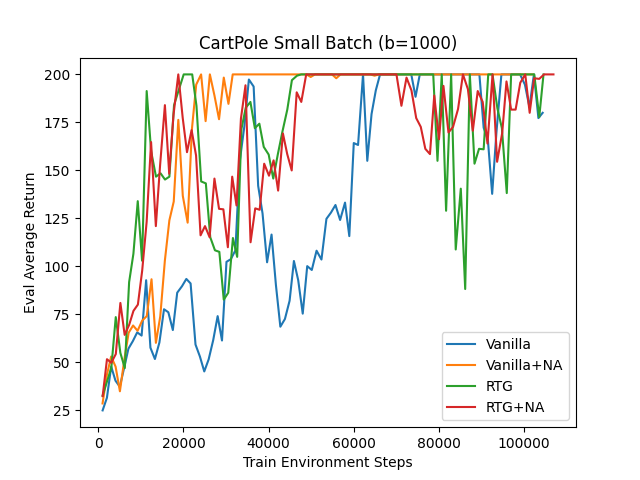
\includegraphics[width=\textwidth]{assets/cartpole_small_batch.png}
        \caption{Small batch (b=1000): Eval Average Return vs.\ environment steps.}
    \end{minipage}
    \hfill
    \begin{minipage}[t]{0.48\textwidth}
        \centering
        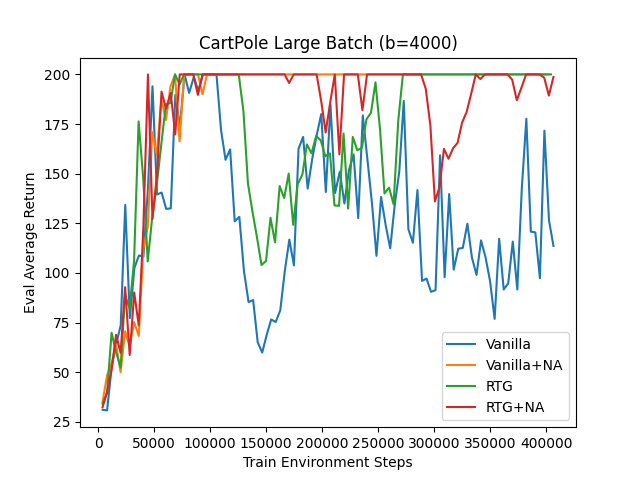
\includegraphics[width=\textwidth]{assets/cartpole_large_batch.png}
        \caption{Large batch (b=4000): Eval Average Return vs.\ environment steps.}
    \end{minipage}
\end{figure}


\subsubsection{Questions:}

Answer the following questions briefly:
\begin{itemize}
    \item Which value estimator has better performance without advantage normalization: the sum of trajectory rewards (REINFORCE) or the one using reward-to-go? \\
    \textbf{Answer:} The reward-to-go estimator should have better performance without advantage normalization. This is because it estimates the return starting from each time step, which provides a more accurate and less noisy estimate of the expected return compared to the sum of trajectory rewards (REINFORCE) that estimates using Monte Carlo return for one trajectory. 
    \item Did advantage normalization help? \\
    \textbf{Answer:} Yes, advantage normalization helps to stabilize training by reducing the variance of the advantage estimates, helping it converge faster and achieve better performance.
    \item Did the batch size make an impact? \\
    \textbf{Answer:} It depends on the configurations, but the effect is not as significant as the other factors. 
    \item Provide the exact command line configurations you used to run your experiments, including any parameters changed from their defaults. \\
    \textbf{Answer:} The following commands were used:
\begin{verbatim}
# Small batch (b=1000)
python cas4160/scripts/run_hw2.py --env_name CartPole-v0 \
    -n 100 -b 1000 --exp_name cartpole
python cas4160/scripts/run_hw2.py --env_name CartPole-v0 \
    -n 100 -b 1000 -rtg --exp_name cartpole_rtg
python cas4160/scripts/run_hw2.py --env_name CartPole-v0 \
    -n 100 -b 1000 -na --exp_name cartpole_na
python cas4160/scripts/run_hw2.py --env_name CartPole-v0 \
    -n 100 -b 1000 -rtg -na --exp_name cartpole_rtg_na

# Large batch (b=4000)
python cas4160/scripts/run_hw2.py --env_name CartPole-v0 \
    -n 100 -b 4000 --exp_name cartpole_lb
python cas4160/scripts/run_hw2.py --env_name CartPole-v0 \
    -n 100 -b 4000 -rtg --exp_name cartpole_lb_rtg
python cas4160/scripts/run_hw2.py --env_name CartPole-v0 \
    -n 100 -b 4000 -na --exp_name cartpole_lb_na
python cas4160/scripts/run_hw2.py --env_name CartPole-v0 \
    -n 100 -b 4000 -rtg -na --exp_name cartpole_lb_rtg_na
\end{verbatim}
\end{itemize}


\section{Using a Neural Network Baseline}
\label{sec:nn_baseline}

\subsection{Neural Network Baseline Result}

\subsubsection{Plot (Baseline Loss, Eval Average Return):}

\begin{figure}[H]
    \centering
    \begin{minipage}[t]{0.48\textwidth}
        \centering
        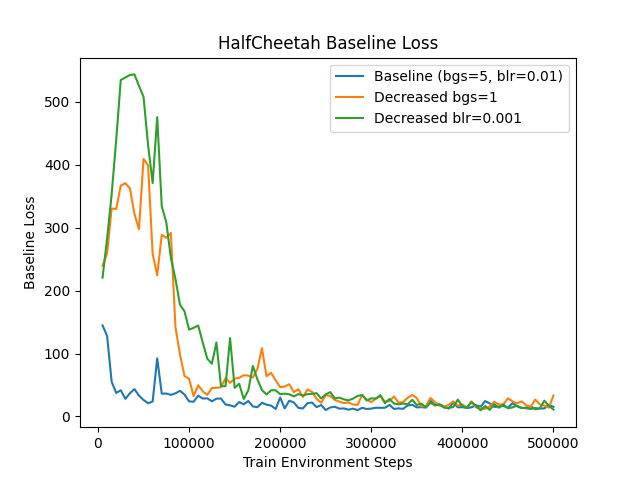
\includegraphics[width=\textwidth]{assets/cheetah_baseline_loss.png}
        \caption{Baseline loss learning curve for HalfCheetah-v4, comparing different baseline gradient steps and learning rates.}
    \end{minipage}
    \hfill
    \begin{minipage}[t]{0.48\textwidth}
        \centering
        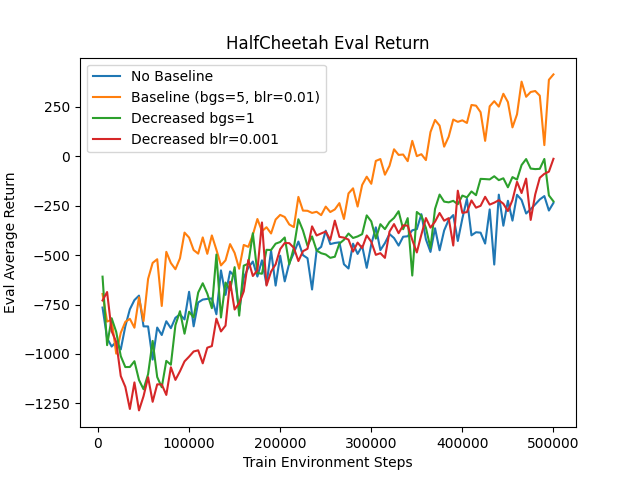
\includegraphics[width=\textwidth]{assets/cheetah_eval_return.png}
        \caption{Eval average return for HalfCheetah-v4, comparing no baseline, standard baseline, and reduced baseline settings.}
    \end{minipage}
\end{figure}

\begin{figure}[H]
    \centering
    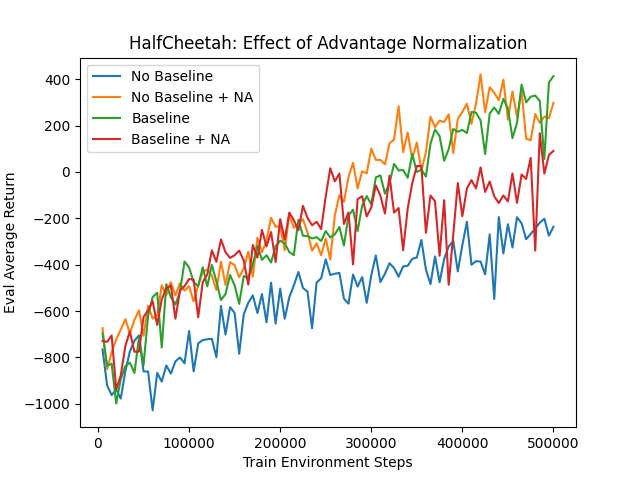
\includegraphics[width=0.7\textwidth]{assets/cheetah_na_comparison.png}
    \caption{Effect of advantage normalization on Eval Average Return for HalfCheetah-v4, comparing baseline and no-baseline variants with and without \texttt{-na}.}
\end{figure}


\subsubsection{Questions:}

Answer the following questions briefly:
\begin{itemize}
    \item Run another experiment with a decreased number of baseline gradient steps (\texttt{-bgs}) and/or baseline learning rate (\texttt{-blr}). How does this affect (a) the baseline learning curve and (b) the performance of the policy? \\
    \textbf{Answer:} We ran two additional experiments: one with decreased gradient steps (\texttt{-bgs 1}) and one with a decreased learning rate (\texttt{-blr 0.001}), compared to the default (\texttt{-bgs 5}, \texttt{-blr 0.01}).
    \begin{itemize}
        \item[(a)] \textbf{Baseline learning curve:} Both reduced settings result in a slower-converging and higher baseline loss, since fewer gradient steps and a smaller learning rate limit how quickly the value network can fit the target Q-values. The baseline remains a poor estimator of $V^\pi(s)$ for longer, leading to noisier advantage estimates.
        \item[(b)] \textbf{Policy performance:} The degraded baseline directly hurts the policy. With \texttt{-bgs 1}, the smoothed eval return stays around $-154.7$ at the end of training (vs.\ $333.2$ for the default). With \texttt{-blr 0.001}, the smoothed return reaches $-73.9$. In both cases, the inaccurate baseline fails to reduce advantage variance effectively, resulting in noisy policy gradient updates and significantly worse final performance.
    \end{itemize}
\end{itemize}


\section{Generalized Advantage Estimator}
\label{sec:gae}

\subsection{GAE Result}
\subsubsection{Plot (Eval Average Return with different $\lambda$):}

\begin{figure}[H]
    \centering
    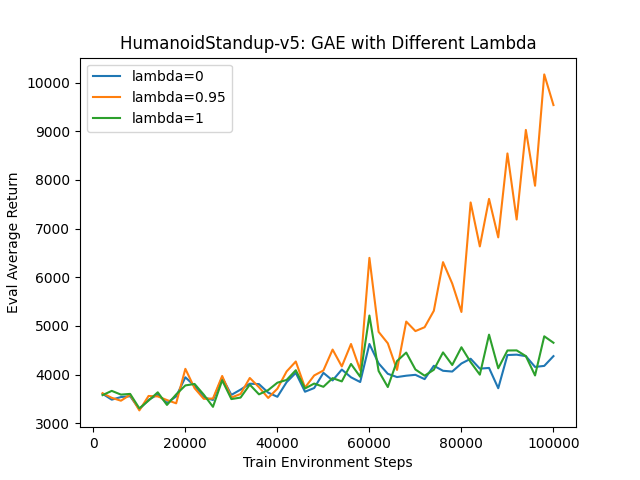
\includegraphics[width=0.7\textwidth]{assets/gae_humanoid.png}
    \caption{Eval Average Return on \texttt{HumanoidStandup-v5} for GAE with $\lambda \in \{0, 0.95, 1\}$.}
\end{figure}

\subsubsection{Questions:}

Answer the following questions briefly:
\begin{itemize}
    \item Describe in words how $\lambda$ affected task performance. \\
    \textbf{Answer:} $\lambda=0.95$ achieved the best performance, reaching an eval return of approximately $9537$ by the end of training and still trending upward. $\lambda=1$ performed comparably in the early stages but showed more variance. $\lambda=0$ performed the worst, plateauing around $4000$. This is because $\lambda=0.95$ strikes a good balance between bias and variance in the advantage estimates: it incorporates enough multi-step information to provide a meaningful learning signal while discounting distant rewards to keep variance manageable. In contrast, $\lambda=0$ produces advantages close to zero once the baseline fits well (TD errors vanish), leaving almost no gradient signal for the policy.

    \item Consider the parameter $\lambda$. What does $\lambda=0$ correspond to? What about $\lambda=1$ ? Relate this to the task performance in \texttt{HumanoidStandup-v5} in one or two sentences. \\
    \textbf{Answer:} $\lambda=0$ reduces GAE to a one-step TD error $A_t = r_t + \gamma V(s_{t+1}) - V(s_t)$, which is low variance but high bias when the value function is imperfect. $\lambda=1$ reduces GAE to the full Monte Carlo return minus the baseline $A_t = \sum_{t'=t}^{T} \gamma^{t'-t} r_{t'} - V(s_t)$, which is unbiased but high variance. In \texttt{HumanoidStandup-v5}, $\lambda=0$ severely limits learning because a well-fitted baseline nearly cancels the TD errors, producing near-zero advantages and stalling policy updates, while $\lambda=1$ introduces too much variance from the long horizon. The intermediate $\lambda=0.95$ achieves the best performance by balancing these two extremes.
\end{itemize}


\section{Proximal Policy Optimization}
\label{sec:ppo}

\subsection{PPO Result}
\subsubsection{Plot (Eval Average Return for PPO and the baseline):}

\begin{figure}[H]
    \centering
    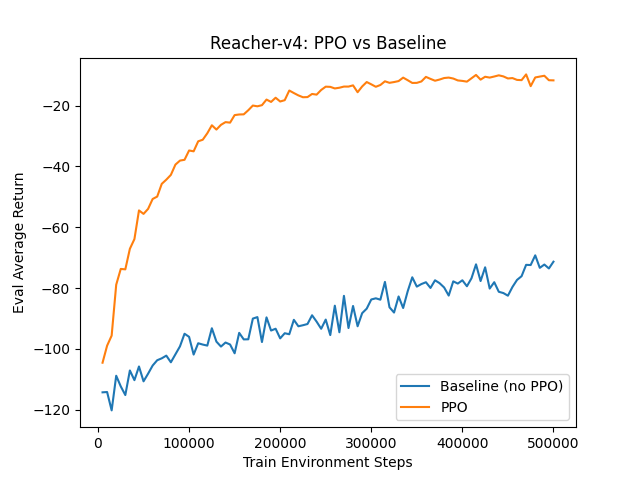
\includegraphics[width=0.7\textwidth]{assets/reacher_ppo.png}
    \caption{Eval Average Return on \texttt{Reacher-v4} for PPO vs.\ the baseline (vanilla PG with GAE). PPO achieves a best return of $-9.75$ while the baseline plateaus at $-69.25$.}
\end{figure}

\subsubsection{Questions:}

Answer the following questions briefly:
\begin{itemize}
    \item If we do not use surrogate objective and do multiple batch updates, what would happen? Justify the result. \\
    \textbf{Answer:} Without the surrogate objective, performing multiple gradient updates on the same batch is equivalent to running vanilla policy gradient with more steps on stale data. Each update shifts the policy further from the one that collected the data, so the importance ratio $\pi_\theta / \pi_{\theta_k}$ grows large and the gradient estimates become increasingly inaccurate. This causes the policy to overshoot, resulting in destructively large updates that degrade performance and destabilize training. In contrast, PPO's clipping mechanism limits how far the new policy can deviate from the old one at each step, making multiple epochs of minibatch updates safe and improving sample efficiency.
\end{itemize}


%% TODO: Please provide us your feedback on homework 2
\section{Discussion}

Please provide us a rough estimate, in hours, for each problem, how much time you spent. This will help us calibrate the difficulty for future homework.

\begin{itemize}
    \item \textbf{Policy Gradients}: 1 hour
    \item \textbf{Neural Network Baseline}: 2 hours
    \item \textbf{Generalized Advantage Estimator}: 30 minutes
    \item \textbf{Proximal Policy Optimization}: 1 hour
\end{itemize}

Feel free to share your feedback here, if any:
\textbf{\color{red}We would really appreciate your feedback to improve the reinforcement learning class.}


\end{document}

